\section{2D rendering}
The game engine has to be able to display and render images on screen.
The game engine will support 2D games, but how does the game engine render images to the screen?

\subsection{SDL2} \label{SDL2}
A simple way to get graphics working in you own custom application is to use a graphics library.
One of the most used simple 2D graphics libraries is SDL2 \cite{sdl2}.
SDL2 is a library written in C that allows the user to have very easy and lightweight cross-platform rendering capabilities.
SDL2 handles most things, so the user can start SDL2 and load and display images, without having to deal with the OS or GPU.
SDL2 does not only handle rendering images but is also capable of managing audio, keyboard, mouse and joystick, allowing for easy user input and audio management across different platforms.

\subsubsection{SDL2 POC}
For the purpose of research a SDL2 POC was created. In this POC the basics of window, renderer and texture creation are covered.
The POC is an application in which an image could be moved across the screen by using the w,a,s and d, keys.
A screenshot of the POC can be seen in \autoref{fig:poc_SDL2}.

\begin{figure}[h!]
    \centering
    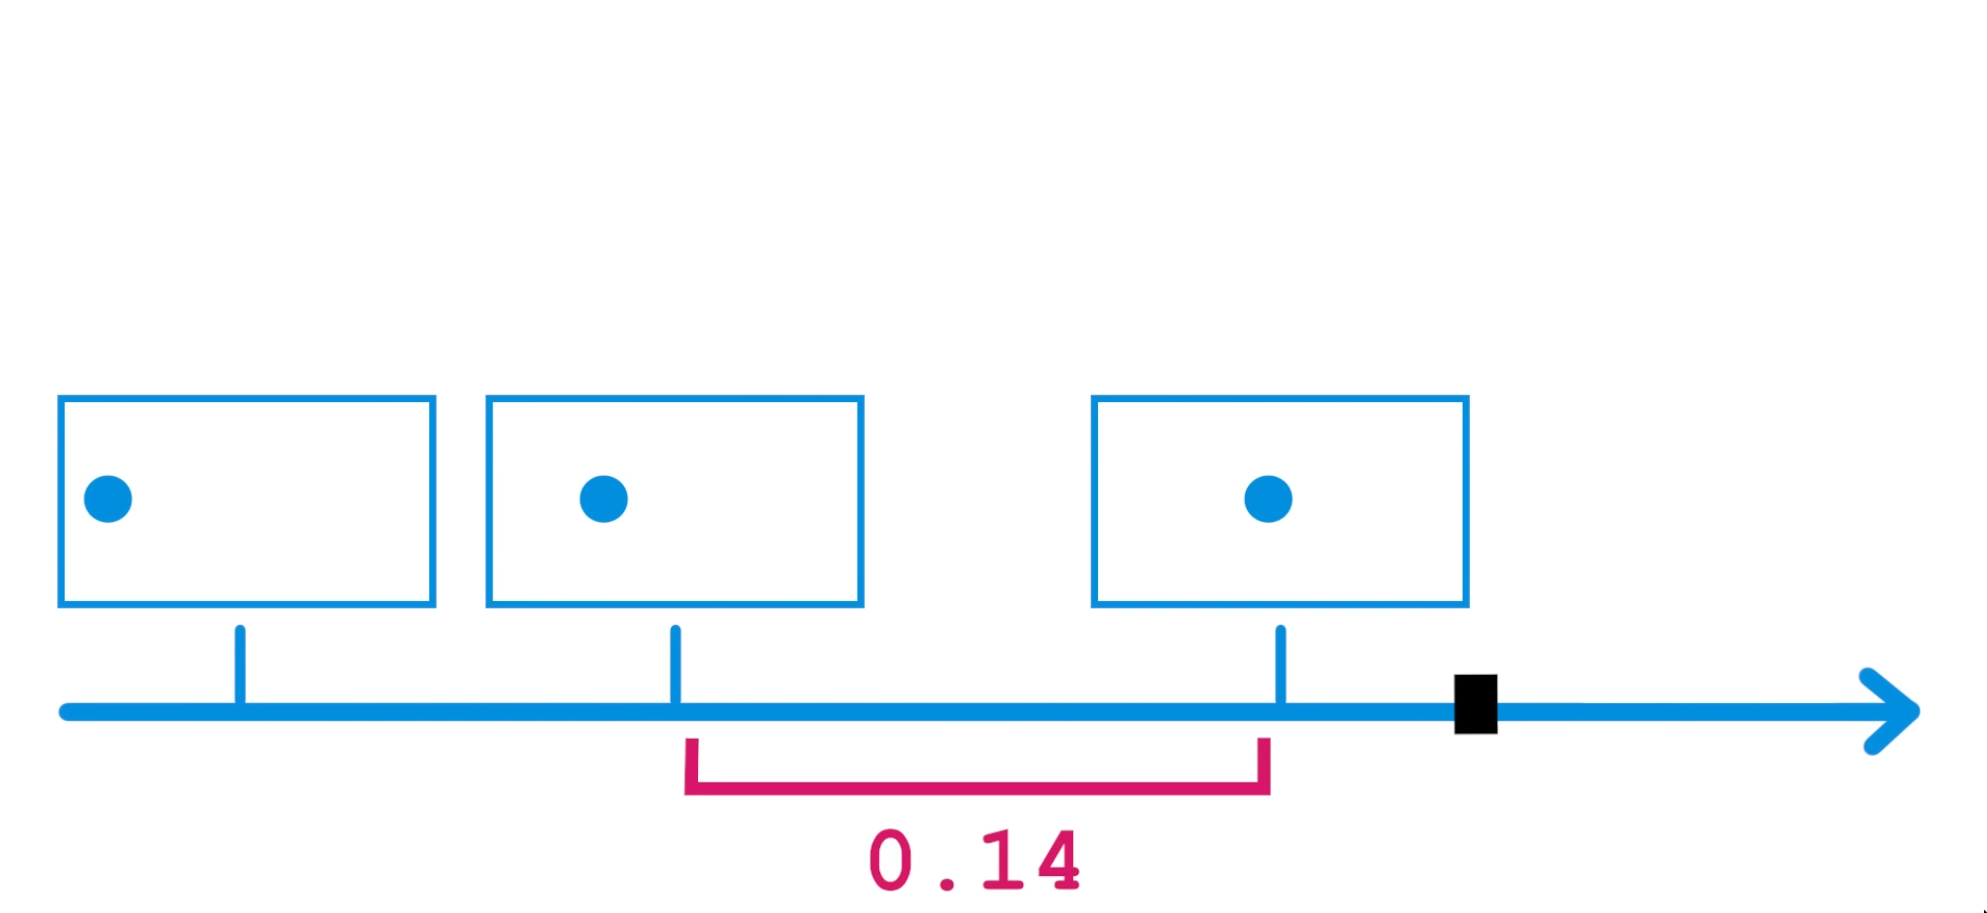
\includegraphics[width=0.7\textwidth]{pos_SDL2_screenshot.png}
    \caption{Screenshot of SDL2 POC}
    \label{fig:poc_SDL2}
\end{figure}

\subsection{Cairo}
Like SDL2 Cairo \cite{cairo}  offers a library written in C that allows the user to render text and images to the screen in a simple way.
Unlike SDL2 Cairo does not offer any access to sound, keyboard, mouse and joystick.
Cairo does not offer these features because the library is meant to be graphics only and as small as possible.

\subsection{OPENGL}
OPENGL \cite{opengl} is not a graphics library but is a shader language, which means that is it a programming language that is compiled to run on the GPU for rendering graphics.
Libraries like SDL2 \cite{sdl2} use OPENGL to render the textures to the screen.
Directly working with OPENGL gives the developer exact control over the render process, textures and effects on screen.
But this exact control comes with way more needed knowledge and development time than using SDL2 which has all the GPU related code under the hood.
